% !TeX spellcheck = cs_CZ
% Basis of Linear Algebra:
{\tikzset{external/prefix={tikz/MAI/}}
 \tikzset{external/figure name/.add={ch02_}{}}
%---------------------------------------------------------------------------------------------------
% intro_linear_algebra.tex
%---------------------------------------------------------------------------------------------------
% ==================================================================================================
% In linear algebra, a basis is a set of linearly independent vectors that, in a
% linear combination, can represent every vector in a given vector space or free
% module, or, more simply put, which define a "coordinate system".[1] In more
% general terms, a basis is a linearly independent spanning set. 
% --------------------------------------------------------------------------------------------------
\chapter{Základy lineární algebry}\label{mai:IchapII}
\minitoc
  \section{Všemocná úměra aneb lineární algebra poprvé}
    Tuto kapitolu bychom mohli opatřit podtitulem \emph{„To nejnutnější z lineární algebry“}. 
    Dovíme se v ní, co je třeba si představit pod pojmem \emph{„linearita“}, najdeme příklady 
    linearity v geometrii i v přírodovědě (fyzice, chemii, biologii) a formulujeme základní 
    poznatky týkající se řešení soustav lineárních rovnic. Do této oblasti patří i počítání s 
    vektory a maticemi — objekty, které jsou velmi vhodné k vyjádření fyzikálních veličin.
    
    \subsection{Lineární rovnice}
      Co tedy znamená slovo \textbf{linearita}? Pochází z latiny, \emph{linea recta = přímka}, 
      česky bychom řekli \emph{přímá úměrnost} nebo jen jednoduše \emph{úměra}.
      
      Nejjednodušší příklady linearity patří do oblasti geometrie — vyjádření \emph{přímek} a 
      \emph{rovin}. Jistě si ze střední školy vzpomínáme, že body těchto útvarů popisujeme jejich 
      souřadnicemi na přímce \(\mathcal{R}\), v rovině \(\mathcal{R}^2\), v prostoru 
      \(\mathcal{R}^3\). Souřadnice bodu v rovině tedy tvoří \emph{uspořádanou dvojici} reálných
      čísel, v prostoru pak \emph{uspořádanou trojici} reálných čísel. (Pozor, dvojice \([a, b]\) a 
      \([b, a]\) představují různé body.)

      %---------------------------------------------------------------
        % !TeX spellcheck = cs_CZ
% Musilova2009MA1

\begin{example}\label{mai:exam001}
  \textbf{Parametrické vyjádření přímky}\newline
  \emph{Přímka} — jednorozměrný lineární útvar v jednorozměrném prostoru \(\mathcal{R}^1\), 
  dvojrozměrném prostoru \(\mathcal{R}^2\), trojrozměrném prostoru \(\mathcal{R}^3\) (nebo i 
  n-rozměrném prostoru \(\mathcal{R}^n\)), je určena dvěma body, třeba \(A\) a \(B\), nebo
  ekvivalentně, bodem \(A\) a \emph{směrovým} vektorem \(\vec{u}\) (obr. \ref{mai:fig000}). 
  Je-li \(X\) obecným bodem na této přímce, je vektor \(\overrightarrow{AX}\) rovnoběžný, tj. 
  \emph{kolineární}, se směrovým vektorem \(\vec{u}\). (Jako směrový můžeme samozřejmě 
  použít i vektor \(\overrightarrow{AB}\).) Vektor \(\overrightarrow{AX}\) má tedy s vektorem 
  \(\vec{u}\) stejný směr, lišit se může velikostí nebo orientací. Tuto skutečnost zapíšeme 
  tak, že \(\overrightarrow{AX}\) je \emph{t}-násobkem vektorů \(\vec{u}\),
  \begin{equation*}
  \overrightarrow{AX} = t \cdot \vec{u}.
  \end{equation*}
  {\centering
    \captionsetup{type=figure}
    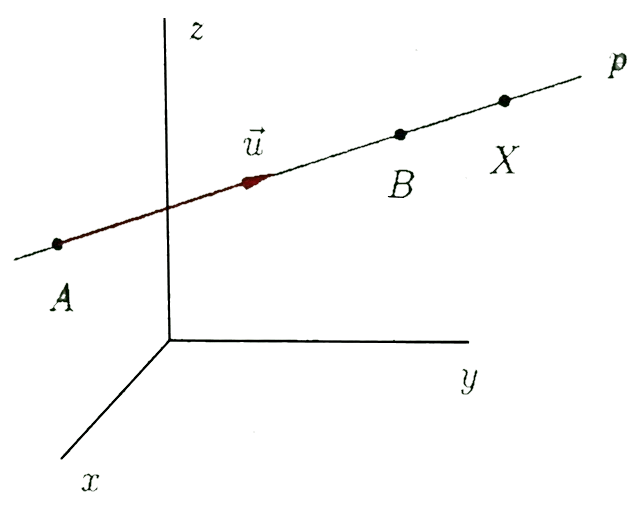
\includegraphics[width=0.5\linewidth]{mai_fig000.png}
    \captionof{figure}{Zadáni přímky. \cite[s.~1]{Musilova2009MA1}
    \label{mai:fig000}}
    \par}        
  Veličinou \(t\), takzvaným \emph{parametrem}, který může nabývat všech reálných hodnot, 
  \(t\in\mathcal{R}\), dokážeme popsat všechny vektory \(\overrightarrow{AX}\), jejichž 
  koncový bod \(X\) leží na přímce \(p\). Naopak, žádné jiné body \(X\) než ty, které leží na 
  přímce \(p\), tuto vlastnost nemají. S označením bodů \(A\), \(X\), resp. vektorů 
  \(\vec{u}\), \(\overrightarrow{AX}\) kartézskými souřadnicemi, resp. složkami
  \begin{align*}
                    A &= (x_A,y_A, z_A), \\ 
                    X &=(x,y,z),         \\
              \vec{u} &= (u_1,u_2,u_3),  \\ 
  \overrightarrow{AX} &= (x - x_A, y - y_1A, z-z_A),
  \end{align*}
  dostáváme \textbf{parametrické vyjádřeni přímky} \(p\) ve tvaru
  \begin{equation}
    p = \left\{(x,y,z)\in\mathcal{R}^3\,|\,
    \begin{matrix}
      x = x_A + tu_1,        \\
      y = y_A + tu_2,        \\
     z = z_A + tu_3,
    \end{matrix}
    \;t\in\mathcal{R}
    \right\}. \label{MAI:eq_M001}
  \end{equation}
\end{example}
\normalsize
      %---------------------------------------------------------------
      Vidíme, že kartézské souřadnice bodu na přímce se vůči souřadnicím bodu \(A\) mění přímo 
      úměrně v závislosti na hodnotě parametru \(t\), tj. závisí na jeho první mocnině. Příslušná 
      závislost se nazývá \textbf{lineární funkcí}.
      
      Obdobně zapíšeme parametrické vyjádření roviny v \(\mathcal{R}^3\):
      %---------------------------------------------------------------
      % !TeX spellcheck = cs_CZ

\begin{example}\label{mai:exam004}
  \textbf{Parametrická vyjádření roviny}:\newline
  Rovina v trojrozměrném prostoru \(\mathcal{R}^3\) je zadána třemi body \(A\), \(B\) a \(C\), 
  které nesmějí ležet v jedné přímce, popřípadě dvěma body \(A\) a \(B\) a vektorem v nerovnoběžným 
  s \(\overrightarrow{AB}\), anebo bodem \(A\) a dvěma nerovnoběžnými směrovými vektory \(\vec{u}\) 
  a \(\vec{u}\) (obr. \ref{MAI:FIG002}). Všechny tyto typy zadání jsou ekvivalentní. Lze volit 
  například \(\vec{u} = \overrightarrow{AB}\), \(\vec{v} = \overrightarrow{AC}\). Je-li \(X\) 
  libovolným bodem roviny \(\varrho\), jsou vektory \(\overrightarrow{AX}\), \(\vec{u}\) a 
  \(\vec{v}\) \textbf{lineárně závislé}. To znamená, že existují taková reálná čísla \(r\) a \(s\), 
  že vektor \(\overrightarrow{AX}\) lze zapsat jako lineární kombinaci

  {\centering
    \captionsetup{type=figure}
    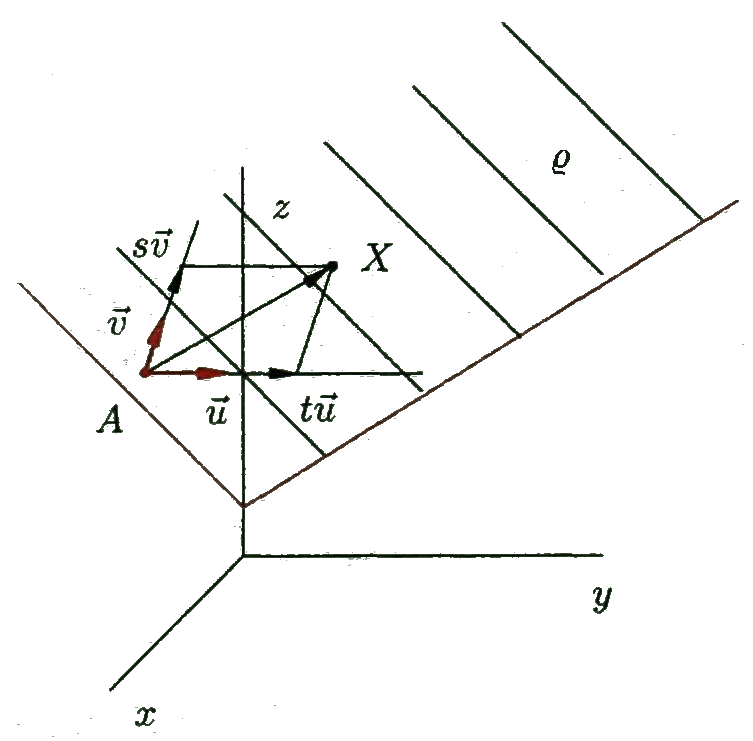
\includegraphics[width=0.5\linewidth]{Musilova_FIG002.png}
    \captionof{figure}{Zadáni roviny. \cite[s.~3]{Musilova2009MA1}}
    \label{MAI:FIG002}
    \par}  
  
\end{example}
  
      %---------------------------------------------------------------
      
    \subsection{Soustavy lineárních rovnic a jejich rychlé řešení}
      Příkladů linearity v přírodě bychom mohli nalézt bezpočet. Vraťme se však k matematice a k 
      problematice uvedené v názvu tohoto odstavce, k soustavám lineárních rovnic. Začněme 
      jednoduchou slovní úlohou ze základní školy:

      %---------------------------------------------------------------
      % !TeX spellcheck = cs_CZ

\begin{example}\label{mai:exam005}
  \textbf{Příklad s ježibabou:}\newline
  Jeníček a Mařenka kradli ježibabě perník. Dohromady snědli 11 perníkových srdíček. Jeníček jich 
  přitom zkonzumoval o 3 více než Mařenka. Otázka je tradiční — kolik srdíček snědl každý z nich?
  Označíme-li \(M\) počet kousků, které snědla Mařenka a \(J\) počet srdíček, na nichž si pochutnal 
  Jenda, můžeme informace zadané v úloze zapsat takto:
    \begin{equation*}
      M + J = 11 \qquad J = M + 3.
    \end{equation*}
  Řešení není problémem, snadno vidíme, že \(M = 4\) a \(J = 7\).
\end{example}
      %---------------------------------------------------------------
      
      O samotné řešení této jednoduché úlohy v tuto chvíli nejde. Pojmenujme si však vztahy, které 
      jsme pro neznámé hodnoty \(M\) a \(J\) ze zadání úlohy dostali. Neznámé vystupují v 
      rovnicích v první mocnině, tedy \emph{lineárně}. Máme \emph{soustavu dvou rovnic} o dvou 
      neznámých \(M\) a \(J\). Úvahu snadno zobecníme: Předpokládejme, že máme neznámé veličiny
      \begin{equation*}
        (x_1, x_2, \ldots, x_n)
      \end{equation*}
      a máme o nich \(m\) informací, které lze zapsat ve tvaru lineárních rovnic (neznámé budou v 
      těchto rovnicích vystupovat v první mocnině),
      \begin{align}
        a_{11}x_1 + a_{12}x_2 + \ldots + a_{1n}x_n &= b_1,     \nonumber           \\
        a_{21}x_1 + a_{22}x_2 + \ldots + a_{2n}x_n &= b_2,     \label{mai:eq002}   \\
        .......................................... &= \ldots   \nonumber           \\
        a_{m1}x_1 + a_{m2}x_2 + \ldots + a_{mn}x_n &= b_m,     \nonumber
      \end{align}
      Soustavu (\ref{mai:eq002}) nazýváme soustavou \(m\) lineárních rovnic o \(n\) neznámých. 
      Označme ji jako \(S\) a pod tímto označením se k ní budeme vracet. Soubory reálných čísel 
      \((a_{ij})\) a \((b_i)\), kde \(1 < i < m\), \(1 \leq j < n\), jsou zadány. Lze je uspořádat 
      do takzvaných \textbf{matic}
      \begin{equation}\label{mai:eq003}
        A =
          \begin{pmatrix}
            a_{11} & a_{12} & \ldots & a_{1n} \\
            a_{21} & a_{22} & \ldots & a_{2n} \\
            \ldots & \ldots & \ldots & \ldots \\
            a_{m1} & a_{m2} & \ldots & a_{mn}          
          \end{pmatrix},
          \overline{B} =
          \begin{pmatrix}
            b_1     \\
            b_2     \\
            \ldots  \\
            b_m 
          \end{pmatrix}
      \end{equation}
      
      Matice \(A\) je typu \(m/n\), má \(m\) řádků a \(n\) sloupců, \(i\) je řádkový index a \(j\) 
      je sloupcový index. Matice \(\overline{B}\) je typu \(m/1\) (\(m\) řádků a jeden sloupec), 
      hovoříme také o sloupcové matici. Soustavu \(S\) můžeme zapsat zkráceně pomocí maticového 
      násobení (podrobněji viz později odstavec \ref{MAI:sec_matice}):
      \begin{equation*}
        A \cdot X = \overline{B}, \qquad \text{nebo}
      \end{equation*}  
      \begin{equation}\label{mai:eq004}
          \begin{pmatrix}
            a_{11} & a_{12} & \ldots & a_{1n} \\
            a_{21} & a_{22} & \ldots & a_{2n} \\
            \ldots & \ldots & \ldots & \ldots \\
            a_{m1} & a_{m2} & \ldots & a_{mn}
          \end{pmatrix}
          \cdot
          \begin{pmatrix}
            x_1     \\
            x_2     \\
            \ldots  \\
            x_m 
         \end{pmatrix}
          =
         \begin{pmatrix}
              b_1     \\
              b_2     \\
              \ldots  \\
              b_m 
            \end{pmatrix}
      \end{equation}
      V tuto chvíli vysvětlíme podstatu maticového násobení jen technicky: Násobit mezi sebou 
      můžeme matici \(A = (a_{ij})\) typu \(m/n\) (levý činitel) a matici \(C = (c_{jk})\) typu 
      \(n/p\) (pravý činitel, činitele nelze zaměňovat). Výsledkem je matice \(D = (d_{ik})\) typu 
      \(m/p\), jejíž prvky se počítají podle předpisu
      \begin{equation}\label{mai:eq005}
        d_{ik} = \sum_{j=1}^{n} a_{ij}\cdot c_{jk}.
      \end{equation}
      
      Z tohoto obecného předpisu vidíme, že levé strany soustavy \(S\) lze interpretovat ve tvaru 
      součinu matice \(A\) typu \(m/n\) s maticí neznámých typu \((n/1)\), výsledkem je matice 
      pravých stran \(\overline{B}\), která je typu \(m/1\). Matice \(A\) se nazývá \textbf{maticí 
      soustavy}. Matice, která vznikne jejím \emph{rozšířením} o sloupec pravých stran, tj.
      \begin{equation}\label{mai:eq006}
        B = (A|\overline{B}) =
        \left(
          \begin{array}{cccc|c}
            a_{11} & a_{12} & \ldots & a_{1n} & b_1    \\
            a_{21} & a_{22} & \ldots & a_{2n} & b_2    \\
            \ldots & \ldots & \ldots & \ldots & \ldots \\
            a_{m1} & a_{m2} & \ldots & a_{mn} & b_m
          \end{array}
        \right)
      \end{equation}
      je pak \textbf{rozšířenou maticí soustavy}. Je-li sloupec pravých stran soustavy tvořen 
      samými nulami, nazývá se soustava \textbf{homogenní}, v opačném případě \textbf{nehomogenní}. 
      Řešením soustavy \(S\) nazýváme každou \(n\)-tici \((x_i, x_2,\ldots, x_n)\), která soustavu 
      \(S\) splňuje. Cílem je najít všechna řešení soustavy \(S\). Abychom řešení nalezli, musíme 
      soustavu upravovat, zjednodušovat. Prováděné úpravy mají vést k jednodušší, avšak 
      ekvivalentní soustavě rovnic, tj. takové, která má naprosto stejný soubor všech řešení jako 
      soustava původní. Takové úpravy nazýváme \textbf{ekvivalentními}. Dvě základní, pomocí nichž 
      lze uskutečnit všechny ostatní, jsou
      \begin{itemize}\addtolength{\itemsep}{-0.5\baselineskip}
        \item vynásobení libovolné, například \(i\)-té, rovnice libovolným \emph{nenulovým} číslem,
        \item přičtení \(i\)-té rovnice vynásobené libovolným číslem k \(l\)-té rovnici.
      \end{itemize}      
      V soustavě lze samozřejmě také měnit pořadí rovnic. Tato úprava je rovněž ekvivalentní. 
      Nevypisujeme ji však zvlášť proto, že ji lze realizovat pomocí vhodně zvolené posloupnosti 
      základních dvou úprav.
      
      Abychom nemuseli soustavu stále opisovat i s neznámými, provádíme obvykle ekvivalentní 
      úpravy jen s maticí \(B = (A|\overline{B})\) (každý řádek této matice představuje jednu 
      rovnici soustavy \(S\)). Může se stát, že soustava má právě \emph{jedno řešení}, jako tomu 
      bylo v  úloze o Mařence a Jeníčkovi. Také nemusí mít \emph{řešení žádné}, jako například 
      soustava \(x + y = 0\), \(x + y = l\) (součet dvou čísel nemůže nabývat současně dvou různých 
      hodnot). A třeba má také řešení \emph{nekonečně mnoho} (řešením soustavy jedné rovnice o dvou 
      neznámých \(x + y = 1\) jsou všechny dvojice tvaru \((x, 1 — x)\), kde \(x\) je libovolné). A 
      může mít soustava \(S\) třeba právě dvě řešení? Prostřednictvím následujícího příkladu 
      ukážeme metodu, která vede velmi rychle k nalezení všech řešení a umožňuje také vyslovit 
      obecné závěry o jejich vlastnostech a počtu. Jedná se o \textbf{Gaussovu eliminační metodu}.
      
 
%--------------------------------------------------------------------------------------------------
  \section{Matice}\label{MAI:sec_matice}
    \begin{definition}\label{def_matice}
      Nechť \(m, n\) jsou přirozená čísla. Jestliže každé uspořádané dvojici \(m,n\). Jestliže každé
      uspořádané dvojici \((m,n)\in \{1,2,\ldots,m\}\times \{1,2,\ldots,m\) přiřadíme prvek
      \(a_{i,j}\in\mathcal{R}\) obdržíme reálnou \href{http://cs.wikipedia.org/wiki/Matice}{matici} 
      typu \(m,n\) nad \(\mathcal{R}\). Čísla jsou indexy, \(i\) je řádkový a \(j\) je sloupcový 
      index.
      
      Matici zapisujeme jako
      \begin{equation}\label{matice_zapis}
        A = \left(a_{ij}\right) =\left(
          \begin{array}{ccc}
            a_{11} & \ldots & a_{1n} \\
            \vdots & \ddots & \vdots \\
            a_{m1} & \ldots & a_{nn}
          \end{array}
        \right)
      \end{equation}
      která má právě \(mn\) prvků \((a_{ij})\) uspořádaných do \(m\) řádků a \(n\) sloupců. Stručně 
      píšeme \(A = (a_{ij})\)
    \end{definition}
  
    \begin{example}
      Matice \(\begin{pmatrix}1&2&3&4\\4&3&2&1\\-1&-1&-1&-1\\-2&-1&0&1\end{pmatrix}\) je čtvercová 
      matice velikosti \(4\times4\). Prvek matice \(a_{23}\) je \(2\).
    \end{example}  
    
    \subsection{Maticová algebra}
      \begin{definition} 
        Součinem matice \(A \in \mathcal{R}_{mn}\) a matice \(B \in \mathcal{R}_{np}\), v uvedeném
        pořadí, je matice \(C \in \mathcal{R}_{mp}\) pro kterou platí:
        \begin{align*}
               C &= AB; \quad C = (cij); \\
               \shortintertext{kde}
          c_{ij} &= \sum_n^{k=1}{a_{ik}b_{kj}};\quad
                     i = 1,\ldots,m; \, j = 1,\ldots,p.
        \end{align*} 
      \end{definition}
      Součin matic \(A\) a \(B\) je definován právě tehdy, když počet sloupců matice \(A\) je roven 
      počtu řádků matice \(B\). Obrázek \ref{LA:fig_LA001a} demonstruje jakým způsobem se 
      dostane prvek, který je ve výsledné matici třeba ve druhém řádku a druhém sloupci, násobením 
      druhého řádku levé matice s druhým sloupcem pravé ze zadaných matic. Stejným způsobem získáme 
      hodnotu prvku \(c_{ij}\) (viz \ref{LA:fig_LA001b}).
%      %----------------------------------
      \begin{figure}[ht!]
        \centering  
        \begin{tabular}{@{}c}
          \subfloat[1. krok]{\label{LA:fig_LA001a}
            %\documentclass[11pt]{standalone}
%  \usepackage{helvet}                        % font
%  \usepackage{xltxtra}                       % fontspec package
%  \usepackage{tikz}  
%  \usetikzlibrary{matrix, arrows}
%  \usepackage{circuitikz}

%\begin{document}

\begin{tikzpicture}

\newcommand{\unit}{0.9cm}
\tikzset{
          node  style    sp/.style={draw,circle,minimum size=\unit},
          node  style    ge/.style={circle,minimum size=\unit}, 
          arrow style   mul/.style={draw,sloped,midway,fill=white}, 
          arrow style  plus/.style={midway,sloped,fill=white},
          yl/.style={},
      }

	\matrix (A) [matrix of math nodes, row sep=-0.5em, column sep=-0.5em, 
               text height=1.5ex, text depth=0.25ex,
			   nodes={node style ge}, left delimiter={(}, right delimiter={)}] at (0,0) {
    a_{11}                          & a_{12}                          & \ldots     & 
    a_{1p}                         \\
    | [node style sp] | {a_{21}}    & | [node style sp] | {a_{22}}    & \ldots     & | [node style 
    sp] | {a_{2p}}   \\
    \vdots                          & \vdots                          & \ddots     & 
    \vdots                         \\
    a_{n1}                          & a_{n2}                          & \ldots     & 
    a_{np}                         \\
  };
    
  \matrix (B) [matrix of math nodes, row sep=-0.5em, column sep=-0.5em, 
               text height=1.5ex, text depth=0.25ex,
			   nodes={node style ge}, left delimiter={(}, right delimiter={)}] at (4.5*\unit,4.5*\unit) {
    b_{11}                          & | [node style sp] | {b_{12}}    & \ldots     & 
    b_{1q}                         \\
    b_{21}                          & | [node style sp] | {b_{22}}    & \ldots     & 
    b_{2q}                         \\
    \vdots                          & \vdots                          & \ddots     & 
    \vdots                         \\
    b_{p1}                          & | [node style sp] | {b_{p2}}    & \ldots     & 
    b_{pq}                         \\
  };
  
  % matrice result
  \matrix (C) [matrix of math nodes, row sep=-0.5em, column sep=-0.5em, 
               text height=1.5ex, text depth=0.25ex,
               nodes={node style ge}, left delimiter={(}, right delimiter={)}] at (4.5*\unit,0) {
    c_{11}                          & c_{12}                            & \ldots     & 
    c_{1q}                       \\
    c_{21}                          & | [node style sp,red] | {c_{22}}  & \ldots     & 
    c_{2q}                       \\
    \vdots                          & \vdots                            & \ddots     & 
    \vdots                       \\
    c_{n1}                          & c_{n2}                            & \ldots     & 
    c_{nq}                       \\
  };

  \draw[blue] (A-2-1.north) -- (C-2-2.north);
  \draw[blue] (A-2-1.south) -- (C-2-2.south);
  \draw[blue] (B-1-2.west)  -- (C-2-2.west);
  \draw[blue] (B-1-2.east)  -- (C-2-2.east);
  \draw[angle 60-angle 60,red](A-2-1) to[in=180,out=90] node[arrow style mul] (x) 
    {\tiny\(a_{21}\times b_{12}\)} (B-1-2);
  \draw[angle 60-angle 60,red](A-2-2) to[in=180,out=90] node[arrow style mul] (y) 
    {\tiny\(a_{22}\times b_{22}\)} (B-2-2);
  \draw[angle 60-angle 60,red](A-2-4) to[in=180,out=90] node[arrow style mul] (z) 
    {\tiny\(a_{2p}\times b_{p2}\)} (B-4-2);
  \draw[red,-angle 60] 
    (x) to node[arrow style plus] {$+$} (y)%
        to node[arrow style plus] {$+\raisebox{.5ex}{\ldots}+$} (z)%
        to (C-2-2.north west);   
  \node [draw, below=5pt] at (A.south) 
    { \tiny\(A\) : \textcolor{red}{\(n\) řádků} \(p\) sloupků};
  \node [draw, above=5pt] at (B.north) 
    { \tiny\(B\) : \(p\) řádků \textcolor{red}{\(q\) sloupků}}; 
  \node [draw, below=5pt] at (C.south) 
    {\tiny\(C=A\times B\) : \textcolor{red}{\(n\) řádků}  \textcolor{red}{\(q\) sloupků}}; 
\end{tikzpicture}
%\end{document}}              \\
          \subfloat[2. krok]{\label{LA:fig_LA001b}
            %\documentclass[11pt]{standalone}
%  \usepackage{helvet}                        % font
%  \usepackage{xltxtra}                       % fontspec package
%  \usepackage{tikz}  
%  \usetikzlibrary{matrix, arrows,decorations}
%  \usepackage{circuitikz}





%\begin{document}
\begin{tikzpicture}

\newcommand{\unit}{0.9 cm}
  \tikzset{
          node  style    sp/.style={draw,circle,minimum size=\unit},
          node  style    ge/.style={circle,minimum size=\unit}, 
          arrow style   mul/.style={draw,sloped,midway,fill=white}, 
          arrow style  plus/.style={midway,sloped,fill=white},
          yl/.style={},
      }

  % defintion of matrices
  \matrix (A) [matrix of math nodes, row sep=-0.9em, column sep=-0.9em, 
               text height=1.5ex, text depth=0.25ex,
			   nodes={node style ge}, left delimiter={(}, right delimiter={)}] at (0,0) {
    a_{11}                       & \ldots & a_{1k}                        & \ldots & 
    a_{1p}                       \\
    \vdots                       & \ddots & \vdots                        & \vdots & 
    \vdots                       \\
    | [node style sp] | {a_{i1}} & \ldots & | [node style sp] | {a_{ik}}  & \ldots & | [node style 
    sp] | {a_{ip}} \\
    \vdots                       & \vdots & \vdots                        & \ddots & 
    \vdots                       \\
    a_{n1}                       & \ldots & a_{nk}                        & \ldots & 
    a_{np}                       \\
  };

  \matrix (B) [matrix of math nodes, row sep=-0.9em, column sep=-0.9em, 
               text height=1.5ex, text depth=0.25ex,
               nodes={node style ge}, 
               left delimiter={(}, right delimiter={)}] at (4.7*\unit,4.0*\unit) {
    b_{11} & \ldots & | [node style sp] | {b_{1j}} & \ldots & b_{1q}  \\
    \vdots & \ddots & \vdots                       & \vdots & \vdots  \\
    b_{k1} & \ldots & | [node style sp] | {b_{kj}} & \ldots & b_{kq}  \\
    \vdots & \vdots & \vdots                       & \ddots & \vdots  \\
    b_{p1} & \ldots & | [node style sp] | {b_{pj}} & \ldots & b_{pq}  \\
  };

  % matrice resultat
  \matrix (C) [matrix of math nodes, row sep=-0.9em, column sep=-0.9em, 
               text height=1.5ex, text depth=0.25ex,
               nodes={node style ge}, left delimiter={(}, right delimiter={)}] at (4.7*\unit,0) {
    c_{11} & \ldots & c_{1j}                           & \ldots & c_{1q} \\
    \vdots & \ddots & \vdots                           & \vdots & \vdots \\
    c_{i1} & \ldots & | [node style sp,red] | {c_{ij}} & \ldots & c_{iq} \\
    \vdots & \vdots & \vdots                           & \ddots & \vdots \\
    c_{n1} & \ldots & c_{nk}                           & \ldots & c_{nq} \\
  };

  % arrows
  \draw[blue] (A-3-1.north) -- (C-3-3.north);
  \draw[blue] (A-3-1.south) -- (C-3-3.south);
  \draw[blue] (B-1-3.west)  -- (C-3-3.west);
  \draw[blue] (B-1-3.east)  -- (C-3-3.east);
  \draw[<->,red](A-3-1) to[in=180,out=90] node[arrow style mul] (x)
    {\tiny\(a_{i1}\times b_{1j}\)} (B-1-3);
  \draw[<->,red](A-3-3) to[in=180,out=90] node[arrow style mul] (y) 
    {\tiny\(a_{ik}\times b_{kj}\)} (B-3-3);
  \draw[<->,red](A-3-5) to[in=180,out=90] node[arrow style mul] (z) 
    {\tiny\(a_{ip}\times b_{pj}\)} (B-5-3);
  \draw[red,->] 
    (x) to node[arrow style plus] {$+\raisebox{.5ex}{\ldots}+$} (y)%
        to node[arrow style plus] {$+\raisebox{.5ex}{\ldots}+$} (z);
      % to (C-3-3.north west);
  \draw[->,red] (z) -- (C-3-3.north west);
  \node [draw, below=5pt] at (A.south) 
    { \tiny\(A\) : \textcolor{red}{\(n\) řádků} \(p\) sloupků};
  \node [draw, above=5pt] at (B.north) 
    { \tiny\(B\) : \(p\) řádků \textcolor{red}{\(q\) sloupků}}; 
  \node [draw, below=5pt] at (C.south) 
    {\tiny\(C=A\times B\) : \textcolor{red}{\(n\) řádků}  \textcolor{red}{\(q\) sloupků}}; 
\end{tikzpicture}
%\end{document}}
        \end{tabular}
        \caption{Postup při maticovém násobení}
      \end{figure}

%--------------------------------------------------------------------------------------------------
    \subsection{Označení prvků matice}
      Prvky matice jsou označeny indexy udávajícími \textbf{řádek} a \textbf{sloupec}, v nichž se 
      prvek nalézá. Prvek v \(i\)-tém řádku a \(j\)-tém sloupci matice \(A\) se obvykle značí 
      \(a_{ij}\). Potom \(i\)-tý řádek matice  obsahuje vodorovnou \(n\)-tici prvků \(a_{i1}, 
      a_{i2}, \ldots,a_{in} \), kde \(i=  1,2,\ldots,m\) a \(j\)-tý sloupec matice obsahuje svislou 
      matici čísel \(a_{1j},a_{2j},\ldots,a_{mj}\), kde \(j = 1,2,\ldots,n\).
  
      V tabulce \ref{LA:tab_basic_matrix} jsou uvedeny nejčastější typy matic, které se v algebře 
      často vyskytují. Jsou to například matice řádkové, sloupcové, diagonální\footnote{Prvky 
      \(a_{ii}\) kde \(i=1,2,\ldots,\min(m,n)\) tvoří hlavní diagonálu. Matice \(\mathbf{D}\) je 
      typu \(m,m\), obecně může mít diagonální matice buď ještě další sloupce, v nichž budou samé 
      nuly, anebo další řádky, v nichž budou opět samé nuly.}, jednotkové\footnote{Jestliže \(m = 
      n\), pak mluvíme o čtvercové matici řádu \(m\).}, nulové, transponované a symetrické.
  
      \begin{table}[!ht]
          \centering
          \renewcommand{\arraystretch}{1.8}   % for the vertical padding
            \begin{tabular}{|l||c@{}|}              
              \hline 
              \textbf{Matice}                    & \textbf{Zápis} \\ \hline\hline
              \ttfamily řádková   \(\mathbf{A}\) &  \(a_1,a_2,\ldots,a_n \)\\
              \ttfamily sloupcová \(\mathbf{B}\) & 
                \(\begin{pmatrix}
                  a_1     \\
                  a_2     \\
                  \vdots  \\
                  a_n
                \end{pmatrix}\)                       \\
              \ttfamily diagonální \(\mathbf{C}\) & 
                \(\begin{pmatrix}
                   a_{11} &    0   & \ldots &   0     \\
                      0   & a_{22} & \ldots &   0     \\
                   \vdots & \vdots & \ddots & \vdots  \\
                      0   &   0    & \ldots & a_{mm}
                \end{pmatrix}\)                       \\
              \ttfamily jednotková \(\mathbf{I}\) &
                \(\begin{pmatrix}
                     1    &    0   & \ldots &   0    \\
                     0    &    1   & \ldots &   0    \\
                   \vdots & \vdots & \ddots & \vdots \\
                      0   &   0    & \ldots & 1
                \end{pmatrix}\)                      \\
              \ttfamily nulová \(\mathbf{0}\) & \((a_{ij}),\quad a_{ij} = 0\,\forall\,i, j\) \\
              \ttfamily transponovaná \(\mathbf{D^T}\) &
                \(\begin{pmatrix}
                  a_{11} & a_{21} & \ldots &  a_{m1}\\
                  a_{12} & a_{22} & \ldots &  a_{m2}\\
                  \vdots & \vdots & \ddots & \vdots \\
                  a_{1n} & a_{2n} & \ldots & a_{mn}
                \end{pmatrix}\)    \\
              \ttfamily symetrická \(\mathbf{S}\) 
              & \((a_{ij}),\quad a_{ij}= a_{ji}\,\forall\,i,j\) \\ \hline
            \end{tabular}
          \caption{Speciální typy matic}\label{LA:tab_basic_matrix}
      \end{table}
    
    
      Matice téhož typu \((m,n)\) nad \(\Re\) budeme značit \(\Re_{m,n}\).
      
      \begin{definition}\label{rovnost_matic}
       (Rovnost matic):  Matice \(\mathbf{A} = \left(a_{ij}\right)\) je rovna matici \(\mathbf{B}=
       \left(b_{kl}\right)\), jsou-li matice stejného typu a stejnolehlé prvky se sobě
       \textbf{rovnají}, tj. \(\mathbf{A} \in \Re_{m,n}, \mathbf{B}\in\Re_{m,n}, a_{ij} = b_{ij}, 
       \forall i\in\lbrace1,2,\ldots,m\rbrace, \forall j\in\lbrace1,2,\ldots,n\rbrace\).
      \end{definition}
      
  %===============================Kapitola: Vektory================================================
  \section{Počítání s vektory}
    \textbf{Vektory} budeme nazývat matice typu \(1/n\) a značit je
    \begin{equation*}
      \vec{u} = (u_1, u_2, \ldots, u_n).
    \end{equation*}
    Takže počítat s nimi již umíme! (V zápisu složek vektoru je vynechán řádkový index. V případě 
    matice s jedním řádkem, takzvané \emph{řádkové matice}, je totiž zbytečný.) Číslům \(u_1\) až 
    \(u_n\) budeme pro tuto chvíli říkat \emph{složky vektoru} \(\vec{u}\). Za chvíli tento pojem 
    ještě upřesníme. Celou řadu pojmů, s nimiž jsme se seznámili při počítání s maticemi, můžeme 
    pro vektory přímo použít. Namísto značení \(\mathcal{M} (1/n)\) budeme pro prostor vektorů 
    používat symbol \((\mathcal{R}^n)\) nebo \(\mathcal{C}^n\) (obvyklý symbol pro množinu 
    uspořádaných \(n\)-tic reálných nebo komplexních čísel).
    
    \subsection{Součiny vektorů}
      Kromě základních operací s vektory, tj. sčítání vektorů a násobení vektoru skalárem, se 
      často používají další operace, které obohacují \emph{strukturu vektorového prostoru}. 
      Zůstaneme u vektorů v trojrozměrném prostoru \(\mathcal{R}^3\) a definujeme si skalární, 
      vektorový a smíšený součin vektorů. Skalární součin vektorů definujeme prostřednictvím 
      geometrické definice jako zobrazení, které uspořádané dvojici vektorů (volných vektorů nebo 
      jejich libovolných umístění) přiřazuje reálný číslo podle předpisu
      
  %===============================Kapitola: Determinanty===========================================
  \section{Determinanty}
    Abychom mohli nadefinovat determinant, budeme muset vědět, jak vypočítat permutaci entice, 
    respektive znaménko permutace.
    \subsection{Permutace}
      \begin{definition}\label{permutace}
        Nechť \(\mathbf{M}\) je libovolná konečná množina. Permutací množiny \(M\) nazýváme 
        zobrazení \(\pi\) množiny \(\mathbf{M}\) na sebe.
      \end{definition}
      
      \begin{example}%(Damlová  Nagy, 1985, str. 34)
        Permutace \(\pi\) množiny \(\mathbf{M}= \lbrace a,b,c,d\rbrace\) je např. zobrazení 
        \(\pi\), definované předpisem:
        \begin{equation}\label{permutace_zadani}
          \pi\left(a\right) = c, \,
          \pi\left(b\right) = d, \,
          \pi\left(c\right) = b, \,
          \pi\left(d\right) = a,
        \end{equation}
        Místo tohoto zápisu se však používá přehlednější zápis ve tvaru matice typu \((2,4)\):
        \begin{equation}\label{LA:eq_perm_exam}
            \begin{pmatrix}
            a & b & c & d \\
            c & d & b & a
            \end{pmatrix}
        \end{equation}
        kde v prvním řádku jsou vypsány všechny prvky množiny \(\mathbf{M}\) (v libovolném pořadí) 
        a ve druhém řádku je pod každým prvkem zapsán jeho obraz v permutaci. Tutéž permutaci však 
        můžeme zapsat ve tvaru matice několika různými způsoby. Například mohou být zapsány takto:
        \begin{equation}
          \begin{array}{cc}
            \begin{pmatrix}
              b & a & c & d \\
              d & c & b & a
            \end{pmatrix},         & 
            \begin{pmatrix}
              d & c & b & a \\
              a & b & d & c
            \end{pmatrix}          \\
            \begin{pmatrix}
              d & c & a & b \\
              a & b & c & d
            \end{pmatrix},         &
            \text{apod.}
          \end{array}
        \end{equation}
      \end{example}

      Zřejmě všechny čtyři uvedené zápisy permutace rov. \ref{LA:eq_perm_exam} ve tvaru matice se 
      liší navzájem pouze pořadím sloupců. Aby bylo možné zapsat každou permutaci množiny 
      \(\mathbf{M}\) ve tvaru rov. \ref{LA:eq_perm_exam} jediným způsobem, je nutné zvolit pevné 
      pořadí prvků množiny \(\mathbf{M}\)  a v zápisu permutace uvádět prvky matice \(\mathbf{M}\)  
      v prvním řádku v tomto pořadí. Avšak známe-li toto pořadí prvků množiny \(\mathbf{M}\), je 
      pak  obvykle zbytečné jej v zápisu permutace uvádět, ale stačí uvést pouze pořadí obrazů, tj. 
      druhý řádek. Zvolíme-li např. v naší množině \(\mathbf{M}\) pevné pořadí prvků \(\lbrace 
      a,b,c,d\rbrace\), pak permutaci rov. \ref{permutace_zadani} zapíšeme jako uspořádanou 
      čtveřici \(\lbrace c,d,b,a\rbrace\).
  
      \begin{definition}\label{def_permutace_ntice}
        Když vytváříme uspořádanou \(n\)-tici navzájem různých prvků \(n\)-prv\-ko\-vé množiny 
        \(\mathbf{M}\), přiřazujeme každému prvku množiny \(\mathbf{M}\) právě jedno přirozené 
        číslo, index příslušného prvku, z množiny prvních \(n\) přirozených čísel.
        \begin{equation}\label{permutace_ntice}
          \pi = \lbrace 1, 2, 3, \ldots, n\rbrace
        \end{equation}
      \end{definition}
  
      Proto každé permutaci uspořádané \(n\)-tice prvků množiny \(\mathbf{M}\) odpovídá jednoznačně 
      permutace příslušných indexů tj. permutace množiny \ref{permutace_ntice} z definice 
      \ref{def_permutace_ntice}. Stačí se tedy omezit při vyšetřování permutací n-prvkové množin 
      na vyšetřování permutací množiny \ref{permutace_ntice}. Permutace \(\pi\) množiny 
      \ref{permutace_ntice} budeme zapisovat jako uspořádané \(n\)-tice \(\left(\pi(1), \pi(2) 
      ,\ldots, \pi(n)\right)\), kde \(\pi(i)\) je číslo z množiny \ref{permutace_ntice}, které 
      permutace \(\pi\) přiřazuje číslu \(i\).

      \begin{example}\label{ex_celk_pocet_permutaci}
        \textbf{Spočítejme celkový počet permutací množiny}. V každé uspořádané \(n\)-tici může být 
        na prvním místě kterákoli z \(n\) cifer, na druhém místě kterákoli ze zbývajících \(n-1\) 
        cifer (kromě té, která je na prvním místě), na  třetím místě každá ze zbývajících \(n-2\) 
        cifer atd. Je tedy celkový počet všech permutací \(n\)-prvkové množiny \(n(n-1)(n-2)\cdot 
        \ldots \cdot2\cdot1\). Toto číslo se zapisuje pomocí symbolu \(n!\) (čti 
        \textbf{n-faktoriál}).
      \end{example}
      
      \begin{definition}\label{def_inv_perm}\textbf{Inverze v permutaci}:
        Inverzí v permutaci \(\left(i_1,i_2,…,i_n \right)\) rozumíme každý výskyt takové dvojice 
        čísel, že větší stojí před menším, tj. vlevo od něj.
      \end{definition}  
   
  %=========================== Kapitola: Vlastní čísla a vlastní vektory ==========================
  \section{Vlastní čísla a vlastní vektory}
    \subsection{Motivace} 
      \textbf{Poznámka}: Je-li \(\mathcal{A} : \mathcal{V} \rightarrow \mathcal{V}\) lineární 
      zobrazení z prostoru \(\mathcal{V}\) do prostoru \(\mathcal{V}\) (nikdy se takové zobrazení 
      nazývá lineárním operátorem), pak je přirozeným požadavkem najít takovou bázi prostoru 
      \(\mathcal{V}\), že je matice zobrazení $\mathbf{A}$ v této bázi co nejjednodušší, např. má 
      následující strukturu
      \begin{equation*}
         \mathbf{A}=
           \left(\begin{array}{ccccc}
             \boxed{A_1}       &             &       &       & 0   \\
                 & \boxed{A_2} &             &       &             \\
                 &             & \boxed{A_3} &       &             \\
                 &             &             &\ddots &             \\
              0  &             &             &       & \boxed{A_k}
            \end{array}
           \right),
     \end{equation*}
     kde \(A_k\) jsou čtvercové matice malého řádu (nejlépe \(1\) nebo \(2\)) a ostatní prvky 
     matice jsou nulové. Problém najít bázi, aby v ní matice zobrazení měla diagonální tvar (kde 
     \(A_k\) jsou skaláry), vede k pojmu vlastní číslo a vlastní vektor matice.

      \begin{definition} 
        Nechť \(\mathbf{A}\in \mathcal{C}^{n,n}\) (matice je čtvercová řádu \(n\)).
        \begin{equation}
          \mathbf{A} = (a_{ij}) =
            \begin{pmatrix}
              a_{11} & a_{12} & \ldots & a_{1n} \\
              a_{21} & a_{22} & \ldots & a_{2n} \\
              \vdots & \vdots & \ddots & \vdots \\
              a_{n1} & a_{n2} & \ldots & a_{nn}
            \end{pmatrix}
        \end{equation}

        Jestliže platí
        \begin{equation}\label{eq:vl_number}
          \mathbf{Au} = \lambda\mathbf{u}
        \end{equation}
        pro jisté komplexní číslo \(\lambda\in\mathcal{C}\)  a jistý nenulový vektor 
        \(x\in\mathcal{C}^n, \mathbf{u}\neq\Theta\), potom číslo \(\lambda\) nazýváme 
        \textbf{vlastním číslem} matice \(\mathbf{A}\) a vektor \(\mathbf{u}\) \textbf{vlastním 
        vektorem} příslušným k tomuto vlastnímu číslu. Množinu všech vlastních čísel nazýváme 
        \textbf{spektrem matice} \(\mathbf{A}\). Pokud rov. \ref{eq:vl_number} rozepíšeme, dostaneme
        \begin{equation}
          \begin{pmatrix}
            a_{11} & a_{12} & \ldots & a_{1n} \\
            a_{21} & a_{22} & \ldots & a_{2n} \\
            \vdots & \vdots & \ddots & \vdots \\
            a_{n1} & a_{n2} & \ldots & a_{nn}
          \end{pmatrix}   \cdot
          \begin{pmatrix}
            u_{1} \\  u_{2} \\ \vdots \\  u_{n} \\
          \end{pmatrix}    =\lambda\cdot
          \begin{pmatrix}
            u_{1} \\ u_{2} \\ \vdots \\ u_{n} \\
          \end{pmatrix}
        \end{equation}
        můžeme ji rovněž psát ve tvaru
        \begin{equation*}
            \begin{pmatrix}
            \setlength{\arraycolsep}{3pt}
              a_{11} -\lambda & a_{12}           & \ldots & a_{1n} \\
              a_{21}          & a_{22} -\lambda  & \ldots & a_{2n} \\
              \vdots          & \vdots           & \ddots & \vdots \\
              a_{n1}          & a_{n2}           & \ldots & a_{nn}-\lambda
            \end{pmatrix} \cdot
          \begin{pmatrix}
            u_{1} \\ u_{2} \\ \vdots \\ u_{n} \\
          \end{pmatrix}  =
          \begin{pmatrix}
              0 \\ 0 \\ \vdots \\ 0 \\
            \end{pmatrix}
        \end{equation*}
      \end{definition}

       Tato soustava rov. je \textbf{homogenní} a stručně ji můžeme zapsat
      \begin{equation}\label{vv_hom_zapis}
        \left(\mathbf{A} - \lambda\mathbf{I}\right) = \mathbf{0}
      \end{equation}
      Homogenní soustava má \emph{netriviální řešení}, právě když je determinant matice soustavy 
      roven  nule, tj. v případě soustavy rov. rov. \ref{vv_hom_zapis} platí
      \begin{equation}\label{vv_hom_reseni}
        |\mathbf{A} - \lambda\mathbf{I}| = \mathbf{0}
      \end{equation}
      Determinant \(A(\lambda)=|\mathbf{A} - \lambda \mathbf{I}|\) nazýváme 
      \textbf{charakteristický polynom} matice \(\mathbf{A}\) - jedná se o polynom stupně \(n\) v 
      proměnné \(\lambda\), který má v oboru komplexních čísel \(n\) kořenů. Rovnici 
      \(A(\lambda)=0\) nazýváme \textbf{charakteristická rovnice matice \(\mathbf{A}\)} - jejími 
      kořeny jsou \textbf{charakteristické hodnoty} (resp. \textbf{vlastní čísla}) 
      \textbf{matice} \(\mathbf{A}\).
            
      \begin{note}
        U vlastních čísel studium pouze reálných matic ztrácí smysl, protože i 
        reálná matice může mít komplexní vlastní čísla. Proto se uvažuje obecná komplexní matice.
      \end{note}
      
      \begin{note}
        Podmínka existence nenulového vektoru \(\mathbf{u} = \Theta\) v definici 
        vlastního čísla je nezbytná: kdyby bylo připuštěno i \(\mathbf{u} = \emptyset\), potom by 
        každé komplexní číslo bylo vlastním číslem a definice by ztratila smysl.
      \end{note}
      
      \begin{note}
        Odpovídá-li matice \(\mathbf{A}\) matici nějakého zobrazení \(\mathcal{A}\), pak každý 
        nenulový vektor z jádra zobrazení \(\ker\mathcal{A}\) je vlastním vektorem příslušným 
        vlastnímu číslu \(\lambda\). Je-li \(\ker\mathcal{A} = \{\Theta\}\) 
        (je-li matice \(\mathbf{A}\) regulární), pak \(\Theta\) není vlastním číslem matice 
        \(\mathbf{A}\).
      \end{note}

      %---------------------------------------------------------------
        % !TeX spellcheck = cs_CZ

\begin{example}\label{mai:exam012}
  Je-li \(\mathbf{P}\) matice ortogonální projekce v prostoru \(\mathcal{R}^3\) na nějaký 
  podprostor \(\mathcal{U}\) (\(\mathcal{U}\) je tedy buď rovina nebo přímka procházející 
  počátkem), pak pro každý vektor \(\mathbf{u}\in\mathcal{U}\) platí \(\mathbf{Pu} = 
  \mathbf{u}\), všechny vektory z \(\mathcal{U}\) (s výjimkou nulového vektoru \(\Theta\)) 
  jsou vlastními vektory matice $\mathbf{P}$ příslušné vlastnímu číslu \(\lambda\). Prostor 
  \(\mathrm{U}^\bot\) je roven jádru projekce (nulovému prostoru matice \(\mathbf{P}\)), 
  a tedy každý vektor z ortogonálního doplňku \(\mathcal{U}\) (s výjimkou \(\Theta\)) je 
  vlastním vektorem příslušným k vlastnímu číslu \(0\).

  {\centering
    \captionsetup{type=figure}
    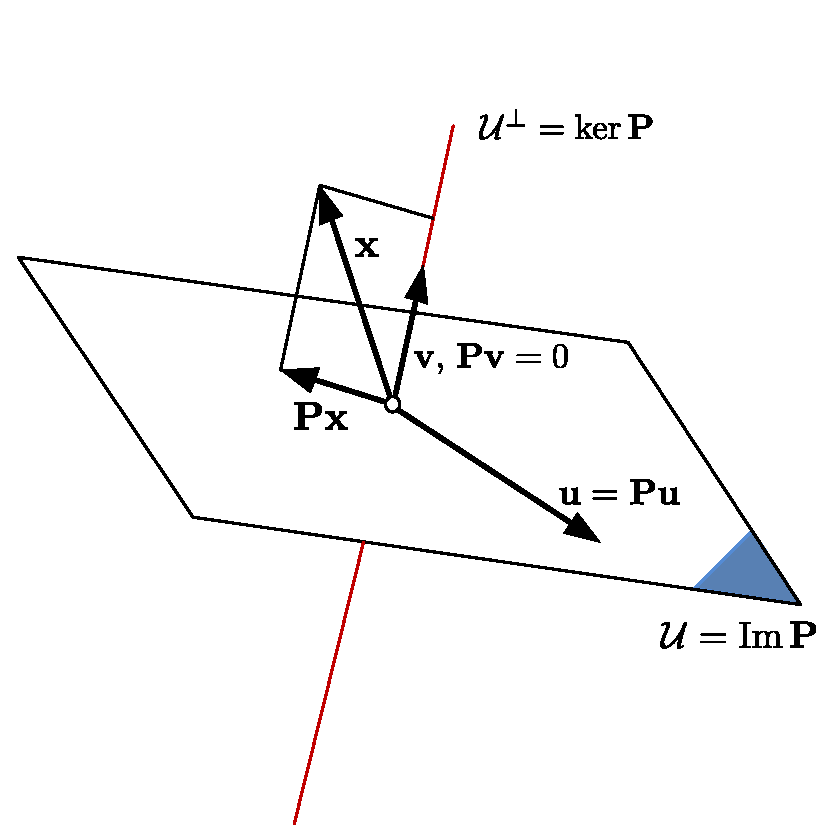
\includegraphics[width=0.7\linewidth]{MAI016.pdf}
    \captionof{figure}{K příkladu \ref{mai:exam012}}
    \label{MAI:FIG016}
    \par}        
\end{example}
      %---------------------------------------------------------------

      %---------------------------------------------------------------
        % !TeX spellcheck = cs_CZ


\begin{example}\label{mai:exam013}
  Určete spektrum matice a její spektrální poloměr následující matice
    \begin{equation*}\label{pr:spektrum_matice}
      \mathbf{A} =
        \begin{pmatrix}
          2  &  2    & 0 \\
         -3  & -3    & 5 \\
          0  & -0.25 & 2
        \end{pmatrix}
    \end{equation*}
  \textbf{Řešení}: Spektrum matice je množina všech jejích vlastních čísel. Spektrální poloměr 
  je maximum z absolutních hodnot vlastních čísel. Vlastní čísla určíme z charakteristické
  rovnice \(\det(\mathbf{A}-\lambda \mathbf{I})=0\).
    \begin{equation*}
      \textbf{A} - \lambda\textbf{I}=
        \begin{pmatrix}
          2-\lambda  &  2          & 0 \\
         -3          & -3-\lambda  & 5 \\
          0          & -0.25       & 2-\lambda
       \end{pmatrix}
    \end{equation*}
    \begin{align}
      \det(\mathbf{A}-\lambda \mathbf{I})                    &= 0           \nonumber\\
      (2-\lambda)
        \begin{pmatrix}
          -3-\lambda  &  5\\
             -0.25    &  2 - \lambda
        \end{pmatrix} -2\cdot
        \begin{pmatrix}
          -3       &  5\\
           0       &  2 - \lambda
        \end{pmatrix}                                        &= 0           \nonumber\\
      (2-\lambda)^2(-3-\lambda)+1.25(2-\lambda)+6(2-\lambda) &= 0           \nonumber\\
      (2-\lambda)[(2-\lambda)(-3-\lambda)+1.25+6]            &= 0           \nonumber\\
      (2-\lambda)(\lambda^2+\lambda+1.25)                    &= 0           \nonumber
    \end{align}
    \begin{equation*}
      \lambda_1 = 2, \quad\lambda_2 = -0.5+i, \quad\lambda_3=-0.5-i
    \end{equation*}
    \begin{itemize}
      \item Spektrum matice \(\mathbf{A}\) je \(\sigma(\mathbf{A})=\{2,-0.5+i,-0.5-i\}\).
      \item Spektrální poloměr \(\rho(\mathbf{A})=\max_i|\lambda_i|=2\).
    \end{itemize}

%    \attachfile[icon=Paperclip, description=Matlab Determine the spectrum of a matrix 
%      and its spectral radius]{../SRC/MAI/matlab/LA001.m}

\end{example}
      %---------------------------------------------------------------

      %---------------------------------------------------------------
        % !TeX spellcheck = cs_CZ
\begin{example}\label{mai:exam014}
  Určete vlastní čísla a vlastní vektory matice \(\mathbf{B} = \mathbf{A}^2 - 4\mathbf{A} + 
  9\mathbf{A}^{-1} - \mathbf{I}\), kde \(\mathbf{A}\) je matice \(\mathbf{A}= 
  \begin{pmatrix}1&0.5\\3.5&4\end{pmatrix}\).

  \textbf{Řešení}: (z předchozího příkladu víme, že \(\lambda_1=4.5, \lambda_2=0.5\)) a
   \(\mathbf{I}\) jednotková matice. Označme symbolem \(\lambda\) vlastní číslo matice 
   \(\mathbf{A}\) a nechť \(\mathbf{x}\) je příslušný vlastní vektor. Pak platí:
   \begin{itemize}
     \item Matice \(\mathbf{A}^2\) má vlastní čísla rovna \(\lambda^2\).
     \item Matice \(4\mathbf{A}\) má vlastní čísla rovna \(4\lambda\).
     \item Matice \(9\mathbf{A}^{-1}\) má vlastní čísla rovna \(\frac{9}{\lambda}\).
   \end{itemize}
   Matice \(\mathbf{B}=\mathbf{A}^2-4\mathbf{A}+9\mathbf{A}^{-1}-\mathbf{I}\) má vlastní čísla 
   ve tvaru  \(\lambda^2-4\lambda+\frac{9}{\lambda}-1\), vlastní vektory jsou stejné jako 
   vlastní vektory odpovídající vlastním číslům matice \(\mathbf{A}\). Tedy:
   \begin{equation*}
       \sigma(B)=\{4.5^2-4\cdot4.5+\frac{9}{4.5}-1,\quad
       0.5^2-4\cdot0.5+\frac{9}{0.5}-1\}=\{3.25, 15.25\}
   \end{equation*}
\end{example}
      %---------------------------------------------------------------


      %---------------------------------------------------------------
       % !TeX spellcheck = cs_CZ

\begin{example}\label{mai:exam002}
  Určete vlastní čísla a odpovídající vlastní vektory následují\-cích matic:
  \begin{equation*}
    \mathbf{A}=
      \begin{pmatrix}
        1   & 0.5\\
        3.5 & 4
      \end{pmatrix}, \quad
    \mathbf{B}=
      \begin{pmatrix}
        3   & -1 \\
        2.5 &  4 
      \end{pmatrix}
  \end{equation*}
  \textbf{Řešení}: Vlastní čísla určíme z charakteristické rovnice: \(\det(\mathbf{A} - 
  \lambda\mathbf{I}) = 0\). Vlastní vektory \(\mathbf{x_i}\) odpovídající vlastním číslům 
  \(\lambda_i\), jsou řešením homogenní soustavy rovnic \((\mathbf{A} - 
  \lambda_i\mathbf{I})\mathbf{x_i} = 0\).
  \begin{itemize}
    \item Vlastní čísla matice \textbf{A}:
      \begin{equation*}
           \textbf{A} - \lambda\textbf{I} =
             \begin{pmatrix}
                1-\lambda  &  0.5          \\
               -3.5        &  4-\lambda
             \end{pmatrix}
      \end{equation*}
      \begin{align*}
         \det(\mathbf{A}-\lambda\mathbf{I}) &= 0 \\
         (1-\lambda)(4-\lambda)-\frac{7}{4} &= 0 \\
         \lambda^2-5\lambda+\frac{9}{4}     &= 0
      \end{align*}
      \begin{equation*}
         \lambda_1 = 4.5,\quad \lambda_2 = 0.5
      \end{equation*}
  \end{itemize}

    \begin{itemize}
      \item Vlastní čísla matice \textbf{B}:
        \begin{equation*}
             \textbf{B} - \lambda\textbf{I}=
               \begin{pmatrix}
                 3-\lambda  & -1             \\
                 2.5        &  4-\lambda
               \end{pmatrix}
        \end{equation*}
        \begin{align*}
           \det(\mathbf{B}-\lambda\mathbf{I}) &= 0 \\
           (3-\lambda)(4-\lambda)+\frac{5}{2} &= 0 \\
           \lambda^2-7\lambda+\frac{29}{2}    &= 0
        \end{align*}
        \begin{equation*}
           \lambda_1 = \frac{7+3i}{2},\quad \lambda_2 = \frac{7-3i}{2}
        \end{equation*}
    \end{itemize}
  % matice A
  Vlastní vektor matice \(\mathbf{A}\) pro \(\lambda_1=4.5: (\mathbf{A} - 
  \lambda_1\mathbf{I})\mathbf{x_1} = 0 \Rightarrow\)
  \begin{align*}
    \begin{pmatrix}
       1  -4.5  &  0.5     \\
      -3.5      &  4-4.5
    \end{pmatrix}
    &\sim
    \begin{pmatrix}
      -3.5  &  0.5         \\
      -3.5  & -0.5
    \end{pmatrix}          \\
    \Rightarrow\mathbf{x_1} &=
    \begin{pmatrix}
      1 \\ 7
    \end{pmatrix}
    \, r, r\in\mathbb{R}, r\neq0
  \end{align*}
  Vlastní vektor matice \(\mathbf{A}\) pro \(\lambda_2=0.5: (\mathbf{A} - 
  \lambda_1\mathbf{I})\mathbf{x_2}=0 \Rightarrow\)
  \begin{align*}
    \begin{pmatrix}
       1  -0.5  &  0.5   \\
      -3.5      &  4-0.5
    \end{pmatrix}
    &\sim
    \begin{pmatrix}
       0.5  &  0.5       \\
       3.5  &  3.5
    \end{pmatrix}        \\
    \Rightarrow\mathbf{x_2} &=
    \begin{pmatrix}
      -1 \\ 1
    \end{pmatrix}
    \, r, r\in\mathbb{R}, r\neq0
  \end{align*}
  % matice B
  Vlastní vektor matice \(\mathbf{A}\) pro \(\lambda_1=\frac{7+3i}{2}: (\mathbf{B} - 
  \lambda_1\mathbf{I})\mathbf{x_1}=0 \Rightarrow\)
  \begin{align*}
    \begin{pmatrix}
       3 - \frac{7+3i}{2}            & -1                                     \\
       \frac{5}{2}                   &  4 - \frac{7+3i}{2}
    \end{pmatrix}
    \sim
    \begin{pmatrix}
      -\frac{1}{2}-\frac{3}{2}i      &  -1                                     \\
      \frac{5}{2}                    & \frac{1}{2}-\frac{3}{2}i
    \end{pmatrix}
    \sim \\
    \begin{pmatrix}
      -\frac{10}{4}                  &-\left(\frac{1}{2} -\frac{3}{2}i\right)  \\
      \frac{5}{2}                    & \frac{1}{2}-\frac{3}{2}i
    \end{pmatrix}
    \sim
    \begin{pmatrix}
      -5                           &-\left(1-3i\right)                         \\
       5                           & \left(1-3i\right)
    \end{pmatrix}
    \rightarrow \\
    \mathbf{x_1}=
    \begin{pmatrix}
      -1+3i \\ 5
    \end{pmatrix}
    \, r, r\in\mathbb{C}, r\neq0
  \end{align*}
  Vlastní vektor matice \(\mathbf{B}\) pro \(\lambda_2=\frac{7-3i}{2}: (\mathbf{B} - 
  \lambda_1\mathbf{I})\mathbf{x_2}=0 \Rightarrow\)
  \begin{align*}
    \begin{pmatrix}
       3  - \frac{7-3i}{2}       &  -1                                     \\
      \frac{5}{2}                &  4 - \frac{7-3i}{2}
    \end{pmatrix}
    \sim
    \begin{pmatrix}
      -\frac{1}{2}+\frac{3}{2}i  &  -1                                     \\
      \frac{5}{2}                & \frac{1}{2}+\frac{3}{2}i
    \end{pmatrix}
    \\sim \\
    \begin{pmatrix}
      -\frac{10}{4}              &-\left(\frac{1}{2} +\frac{3}{2}i\right)  \\
      \frac{5}{2}                & \quad\frac{1}{2}+\frac{3}{2}i
    \end{pmatrix}
    \sim
    \begin{pmatrix}
      -5                         &-\left(1+3i\right)                       \\
       5                         & \quad\left(1+3i\right)
    \end{pmatrix}
    \rightarrow\\
    \mathbf{x_2}=
    \begin{pmatrix}
      -1-3i \\ 5
    \end{pmatrix}
    \, r, r\in\mathbb{C}, r\neq0
  \end{align*}
\end{example}
%---------------------------------------------------------------
\lstinputlisting{../src/MAI/matlab/LA001.m}
\begin{lstlisting}[caption=Výpis programu pro ověření výpočtu vlastních čísel matic programem
  Matlab.]
\end{lstlisting}
%---------------------------------------------------------------
      %---------------------------------------------------------------

  %====================== Kapitola: Polynomy ======================================================
  \section{Polynomy}
      \begin{definition}\label{def_rov_poly}\textbf{Rovnost dvou polynomů}:
        Řekneme, že dva polynomy \(f(x)=a_nx^n+a^{(n-1)}x_{(n-1)}+\ldots+a_1+a_0\) a
        \(g(x)=b_mx^m+b^{(m-1)}x_{(m-1)}+\ldots+b_1+b_0\) stupňů \(n\) a \(m\) se sobě 
        \textbf{rovnají} právě tehdy, když \(m=n\) a \(a_0=b_0\), \(a_1=b_1\), 
        \(a_{(n-1)}=b_{(m-1)}\), \(a_n=b_m\). V tomto případě také říkáme, že mnohočleny \(f(x)\) a 
        \(g(x)\) jsou \textbf{totožné}.
      \end{definition}
      \begin{lemma}\label{la:eq_eqv_poly}
        Jestliže mnohočleny \(f(x)\) a \(g(x)\) jsou dva polynomy stupně \(n\)-tého a jestliže pro 
        \(n+1\) různých reálných nebo komplexních čísel \(x\) platí \(f(x)=g(x)\), potom jsou 
        polynomy \textbf{totožné}.
      \end{lemma}
      
    \subsection{Rozklad ryze racionální funkce na parci\-ální zlomky}

      %---------------------------------------------------------------
       % !TeX spellcheck = cs_CZ
\begin{example}\label{mai:exam015}
  Rozložte na parciální zlomky lomenou racionální funkci \((x):y=\frac{7x+8}{x^2+x-2}\).
  \newline\textbf{Řešení:} Nejprve vypočteme nulové body jmenovatele:
  \begin{align*} 
     x^2+px+q &=(x-u)(x-v) = x^2-(u+v)x+uv            \\
              &\rightarrow p=-(u+v),\quad q=uv
  \end{align*}
  Kořenové činitele  \(x^2+x-2\rightarrow x_1=1, x_2=-2\) zvolíme za jmenovatele parciálních
  zlomků a rozklad hledáme ve tvaru \(\frac{7x+8}{x^2+x-2}=\frac{A}{x-1}+\frac{B}{x+2}\)
  kde \(A\), \(B\) jsou neznámé konstanty. Tyto konstanty určíme tak, aby rozklad platil pro 
  každé \(x\in\mathcal{R}-\{1,-2\}\). Po jednoduché úpravě dostaneme rovnost dvou polynomů
  \(7x+8=(A+B)x+2A-B\). Podle \ref{la:eq_eqv_poly} se musí rovnat koeficienty u \(x\) a absolutní 
  členy obou stran poslední rovnice \(\Rightarrow\) dostaneme soustavu rovnic pro určení \(A\) a 
  \(B\) ve tvaru:
  \begin{align}
    % \nonumber to remove numbering (before each equation)
    7 &= A+B  \nonumber \\ 
    8 &= 2A+B \label{la:eq_parc_example}   
  \end{align}
  dostáváme \(A=5,\quad B=2\). Postup, který jsme užili, nazýváme \textbf{Metodou neurčitých 
  koeficientů}.
  
  Pro určení koeficientů \(A\), \(B\) se užívají také jiné postupy, např. dosazování
  kořenů jmenovatele, která je výhodná zejména v případech, kdy jmenovatel lomené racionální
  funkce má jednoduché kořeny. Postupujeme tak, že rov. \ref{la:eq_parc_example} násobíme
  součinem kořenových činitelů \((x-1)(x+2)=x^2+x-2\) a dostaneme rovnici 
  \(7x+8=A(x+2)+B(x-1)\) pro určení koeficientů \(A\), \(B\) dosazováním kořenů.
    \begin{align*}
      % \nonumber to remove numbering (before each equation)
      x=-2 &\rightarrow       -14+8=B(-2-1)      \rightarrow B=2\\
      x=+1 &\rightarrow  \,\,\,+7+8=A(1+2)\quad  \rightarrow A=5
    \end{align*}
\end{example}
      %---------------------------------------------------------------
      
  %==================== Kapitola: Vektorové prostory ===============================================
  \section{Vektorové prostory se skalárním součinem}
    \subsection{Ortogonální doplňky}
      Nechť \(U\) je podprostor vektorového prostoru \(V\). Ortogonální doplněk $U^\bot$ obsahuje 
      všechny vektory, které jsou kolmé ke každému vektoru z \(U\), neboli \(\forall\vec{v}\in 
      U^\bot\quad \forall\vec{u}\in U\quad \vec{u}\bot\vec{v}\) což lze vyjádřit pomocí skalárního 
      součinu \(\vec{u}\cdot\vec{v} = 0\)
  
      Ortogonální doplněk \(U^\bot\) k podprostoru \(U = \langle\vec{u}_1,\ldots,\vec{u}_k\rangle\) 
      tedy hledáme jako řešení homogenní soustavy rovnic
      \begin{equation*}
        \left(
          \begin{array}{c|c}
             \vec{u}_1  &   0      \\
             \cdots     &  \vdots  \\
             \vec{u}_k  &   0
          \end{array}
        \right),
      \end{equation*}
      nuly na pravé straně při výpočtu zpravidla vynecháváme. Připomeňme také vztah
      \begin{equation}\label{LA:eq_dim_doplnek}
         \dim U + \dim U^\bot = \dim V
      \end{equation}

      %---------------------------------------------------------------
        % !TeX spellcheck = cs_CZ
% Musilova2009MA1

\begin{example}\label{mai:exam011}
  Zjistěte ortogonální doplněk \(\langle(1,-3,2),(2,1,5)\rangle\bot^.\). (Zdroj:
  \cite[s.~3]{MosnaMA3})
  \newline\textbf{Řešení}:
  Hledáme vektor \((x, y, z)\), jehož skalární součin je se zadanými vektory roven nule. Budeme 
  tedy řešit (úpravou na Gaussův tvar pomocí elementárních úprav) homogenní soustavu rovnic
  zadanou maticí
  \begin{equation*}
     \left(
       \begin{array}{ccc|c}
          1  &  -3  & 2 & 0 \\
          2  &   1  & 5 & 0
       \end{array}
     \right)\sim
     \left(
       \begin{array}{ccc|c}
          1  &  -3  & 2 & 0 \\
          0  &   7  & 1 & 0
       \end{array}
     \right)\
  \end{equation*}
  Odtud dostáváme \(z = \alpha\), \(7y + z = 0\) \(\Rightarrow\) \(y = -\frac{1}{7}\alpha\), \(x
  +\frac{3}{7}\alpha + 2\alpha = 0\) \(\Rightarrow\) \(x = -\frac{17}{7}\) neboli 
  \begin{equation*}
  (x, y, z) =\alpha\left(-\frac{17}{7}, -\frac{1}{7}, 1\right) = \alpha(17, 1, -7)
  \end{equation*}

  V dalších příkladech budeme nuly na pravé straně soustavy vynechávat a upravovat na
  výhodnější tvar
  \begin{align*}
       \begin{pmatrix}
          1  &  -3  & 2  \\
          2  &   1  & 5
       \end{pmatrix}
       & \sim
       \begin{pmatrix}
          1  &  -3  & 2 \\
          0  &   7  & 1
       \end{pmatrix}
       \sim                         \\
       \begin{pmatrix}
          1  &   0  & \frac{17}{7}  \\
          0  &   7  & 1
       \end{pmatrix}
       & \sim
       \begin{pmatrix}
          7  &   0  & 17 \\
          0  &   7  & 1
       \end{pmatrix}.
  \end{align*}
  Odtud již snadno zjistíme, že vektor \((x, 1, -7)\) jistě vyhovuje druhé rovnici. Dosadíme-li ho 
  do první rovnice, dostaneme \(7x + 17\cdot(-7) = 0\) a \(x = 17\).

  Hledaný ortogonální doplněk je tedy lineární obal $$\langle(17, 1, -7)\rangle^\bot.$$
  
    {\centering
     \captionsetup{type=figure}
    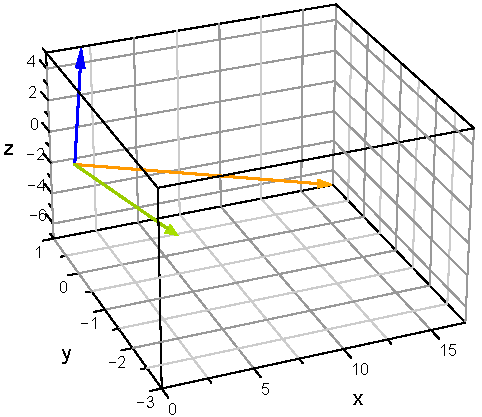
\includegraphics[width=0.8\linewidth]{ort_doplnek_exam01.pdf}
    \captionof{figure}[Ortogonální doplněk]{Vizualizace vektorového prostoru a jeho    
             ortogonálního doplňku pomocí sw MatLab - MuPAD příkazem:\newline
             \texttt{plot(plot::Arrow3d([1,-3,2]), plot::Arrow3d([2,1,5]), 
             plot::Arrow3d([17,1,-7]))}}
    \label{LA:fig_ort01}
    \par}
\end{example}

      %---------------------------------------------------------------
  
      Výsledek předchozího příkladu \ref{mai:exam011} lze interpretovat tak, že jsme našli všechny 
      vektory, které jsou kolmé na rovinu určenou vektory ze zadání. Rovina je útvar       
      dvojrozměrný a protože prostor všech vektorů je trojrozměrný, musí nutně mít podprostor 
      ortogonálních vektorů ve shodě se vztahem \ref{LA:eq_dim_doplnek} pouze jednu dimenzi. Vše 
      je dobře patrné z obr. \ref{LA:fig_ort01}

} % tikzset
%---------------------------------------------------------------------------------------------------
\printbibliography[title={Seznam literatury}, heading=subbibliography]
\addcontentsline{toc}{section}{Seznam literatury}